\documentclass{beamer}
\usepackage[english,russian]{babel}
\usepackage[utf8]{inputenc}
\usepackage{pagenumber}

\usepackage{hyperref}
% Стиль презентации
\usetheme[numbers, totalnumbers]{Dresden}
% цветовая схема
\usecolortheme{beaver}

\makeatletter
\defbeamertemplate*{footline}{Dresden}{
	\leavevmode%
	\hbox{%
	\begin{beamercolorbox}[wd=.2\paperwidth,ht=2ex,dp=1ex,center]{author in head/foot}%
		\usebeamerfont{author in head/foot}%
		\insertauthor	
	\end{beamercolorbox}%
	\begin{beamercolorbox}[wd=0.6\paperwidth,ht=2ex,dp=1ex,center]{title in head/foot}%
		\usebeamerfont{title in head/foot}\inserttitle
	\end{beamercolorbox}%
	\begin{beamercolorbox}[wd=.2\paperwidth,ht=2ex,dp=1ex,right]{date in head/foot}%
		\usebeamerfont{date in head/foot}\hspace*{2em}
		\insertframenumber{} / \inserttotalframenumber\hspace*{2ex}
	\end{beamercolorbox}}%
}
\makeatother

\begin{document}
\title{Хаос в Солнечной системе: обзор}  
\author{Волков Д.В.}
\institute{Санкт-Петербургский государственный университет }
\date{Cолнечная система, семинар \today} 
% Создание заглавной страницы
\frame{\titlepage} 

\begin{frame}{О чем пойдет речь}
        \begin{itemize}
		\item Динамический (детерминированный) хаос 
		\item Исследования самых различных исследовательских групп за последние десятилетия 
		\item Критерии хаоса и границы между регулярной, но сложной динамикой и хаосом. Что делать, если имеем дело с хаосом? Какие методы можно применять, а какие нельзя?
	\end{itemize}

	\begin{equation}
		\Phi = O * p - M + y (\lambda - a)
	\end{equation}
\end{frame}

\begin{frame}{Терминология и определения}
Предметом исследования качественной теории являются, главным образом, сосредоточенные системы, описываемые набором обыкновенных ДУ
\begin{equation}
        \frac{dx}{dt} = v(x, a)
\end{equation}
где $x(t) = {x_1, x_2, \ldots, x_n}$ - совокупность динамических переменных, $v$ - векторная функция заданной гладкости $r$, определенная в некоторой области $M$, которую называют фазовым подпространством системы, $a$ -- параметр.
\end{frame}


\begin{frame}{Терминология и определения}
\begin{itemize}
        \item        Одним из ключевых понятий при изучении динамических систем является понятие грубости (или структурной устойчивости), введенное А.А.Андроновым и Л.С.Понтрягиным. 
        \item Предельные циклы -- замкнутые фазовые траектории, отвечающие периодическому движению.

\end{itemize}
\end{frame}


\begin{frame}{Терминология и определения}
        \textbf{Аттаракторы} -- компактное подмножество $A$ фазового пространства $M$, которое удовлетворяет следующим условиям:
                \begin{itemize}
                        \item Инвариант относительно потока динамической системы (попав на аттрактор, мы остаёмся там сколь угодно долго)
                        \item Существует окрестность $U$, которая сжимается к $A$ под действием потока (существование области притяжения аттрактора, т.е. о совокупности начальных точек таких, что фазовые траектории при $t \infty$ стремятся к $A$)
                        \item $A$ нельзя разложить на два и более непересекающихся инвариантных множества (нужно, чтобы исключить аттракторы, состоящие из нескольких отдельных компонент)
                \end{itemize}
\end{frame}


\begin{frame}{Терминология и определения}
        Даём определение \textbf{хаосу}.
                \begin{itemize}
                        \item Экспоненциальная чувствительность системы к заданию начальных условий или к внешним воздействиям
                        \item Наличие транзитивности (неразложимость)
                        \item Наличие плотности периодических орбит
                        \item Сложность траектории
                        \item Физично -- через энтропию и размерности
                        \item Неотличимость от некоторого случайного процесса
                \end{itemize}
                Позднее выяснилось, что первое -- избыточно (!). Ссылки ниже.
                Практически любая типичная нелинейная система более чем с одной степенью свободы может проявлять хаотические свойства.
\end{frame}


\begin{frame}{Вопрос}
        Является ли длина стержня рациональным или иррациональным числом? (интересует только качественное свойство стержня)

        Также см. \textbf{теорию бильярдов}. 
\end{frame}


\begin{frame}{Терминология и определения}
        \textbf{Время Ляпунова} -- время, за которое система приходит к состоянию хаоса, определенному выше. Определяется как число, обратное к наибольшему из показателей Ляпунова (которые в свою очередь характеризуют степень растяжения и сжатия в системе вдоль устойчивых и неустойчивых направлений).

\end{frame}


\begin{frame}{В Солнечной системе}
        Были выбраны по вкусу и из других субъективных соображений следующие работы:
        \begin{itemize}
                \item The Origin of Chaos in the Outer Solar System (Murray+1999)
                \item The role of chaotic resonances in the solar system (Murray+2001)
                \item Chaos in the Solar System (Lecar+2001)
                \item Is the outer Solar System chaotic? (Wayne B. Hayes 2007)
                \item Theory of Secular Chaos and Mercury's Orbit (Lithwick+2010)
                \item Secular chaos and its application to Mercury, hot Jupiters, and the organization of planetary systems (Lithwick+2013)
                \item Chaos in some young asteroid families (Rosaev+2016)
        \end{itemize}
\end{frame}




\begin{frame}{The Origin of Chaos in the Outer Solar System (1999)}
        \textbf{Авторы}: N. Murray (Toronto) and M.Holman (Cambridge).

        \textbf{Кратко}: Классические аналитические теории солнечной системы указывают на её стабильность, но численные эксперименты показывают, что она хаотична. Это противоречие разрешилось аналитическими средствами в пользу последней точки зрения. На примере Урана демонстрируется, что хаос среди планет-гигантов это следствие наложения резонансов среди Юпитера, Сатурна и Урана, и даются оценки времени Ляпунова (около 10 Млет). Время входа в резонансы -- после исчезновения газа и большинства планетезималей в протопланетном диске.
\end{frame}

\begin{frame}{The Origin of Chaos in the Outer Solar System (1999)}
        \begin{itemize}
                \item Аналитическая теория представлена выводом некоторых орбитальных резонансов модели двух и трех тел, c оценками стохастических параметров
                \item Выявлена хаотическая природа потенциала возмущений, которые испытывает Уран со стороны других планет
                \item Резонанс $2:5$ играет важную роль в создании хаоса среди внешних планет, ограничивает возможность их нахождения в солнечной системе в далеком будущем
        \end{itemize}
\end{frame}

\begin{frame}{The Origin of Chaos in the Outer Solar System (1999)}
        Численные эксперименты
        \begin{itemize}
                \item Использовали симплектический интегратор для вычисления движения четырех внешних планет (упростили для уединения эффектов больших планет)
                \item Ляпуновское время составило 7 Млет
        \end{itemize}
\end{frame}

\begin{frame}{The Origin of Chaos in the Outer Solar System (1999)}
        Вокруг современного значения $a_U$:
\begin{figure}[h]
\begin{minipage}[h]{0.7\linewidth}
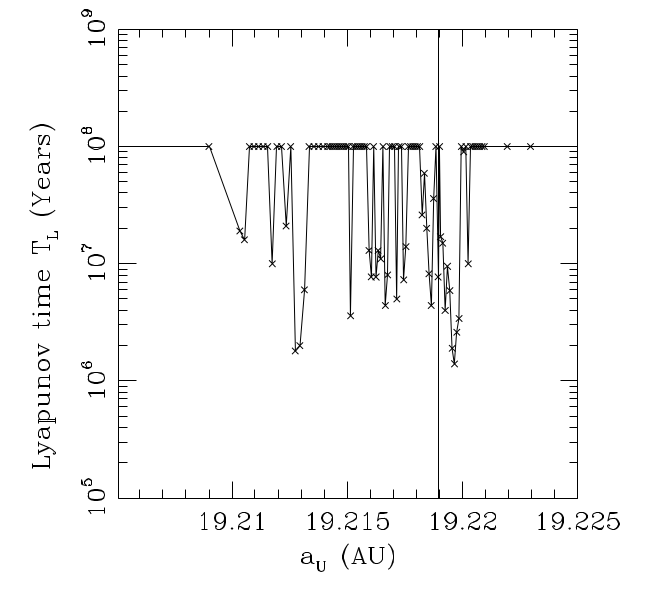
\includegraphics[width=1\linewidth]{./au2_99.png}
\end{minipage}
\end{figure}
\end{frame}

\begin{frame}{The role of chaotic resonances in the solar system (2001)}
        \textbf{Авторы}: N. Murray (Toronto) and M.Holman (Cambridge).

        \textbf{Кратко}: Внешняя и внутренняя солнечная система хаотичны независимо друг от друга. В последнее время среди открытых внесолнечных планетных систем есть проявляющие хаос. Экстремальные проявления -- дестабилизация орбит, неблагоприятные условия для возникновения и существования жизни. Всякая философия и не только.
\end{frame}


\begin{frame}{The role of chaotic resonances in the solar system (2001)}
        В работе рассмотрены:
        \begin{itemize}
                \item \textbf{Люkи Кирквуда} (как резонансы $2:1$ и $3:1$). Подробно исследуется их происхождение.
                        \item Хаос в \textbf{спин-орбитальном} резонансе. Самый <<драматический и важный>> по мнению авторов пример проявления хаоса в динамике планетных систем. Здесь причины в резонансе между вращательным движением планеты и периодом орбитальной прецессии. Асферичность и несимметричность планетных пар. Спутник Сатурна Гиперион -- выделился. Неприятный (но маловероятный) наклон до 90 град земной оси.
        \end{itemize}
\end{frame}

\begin{frame}{The role of chaotic resonances in the solar system (2001)}
        В работе рассмотрены: (продолжение)
        \begin{itemize}
                \item \textbf{Трехтельный} резонанс. Исследования движения астероидов главного пояса показали, что часть этих тел имеют хаотические орбиты с временами Ляпунова порядка $10^5$ лет, причем это движение не вызвано каким-либо резонансом двух тел. Резонансы пропорциональны произведению масс двух взаимодействующих тел.
                \item Этот резонанс является, например, причиной миграции астероидов из внутреннего края пояса к Земле и Марсу. Характерные времена диффузии на несколько порядков меньше возраста солнечной системы.
        \end{itemize}
\end{frame}


\begin{frame}{The role of chaotic resonances in the solar system (2001)}
\begin{figure}[h]
\begin{minipage}[h]{0.7\linewidth}
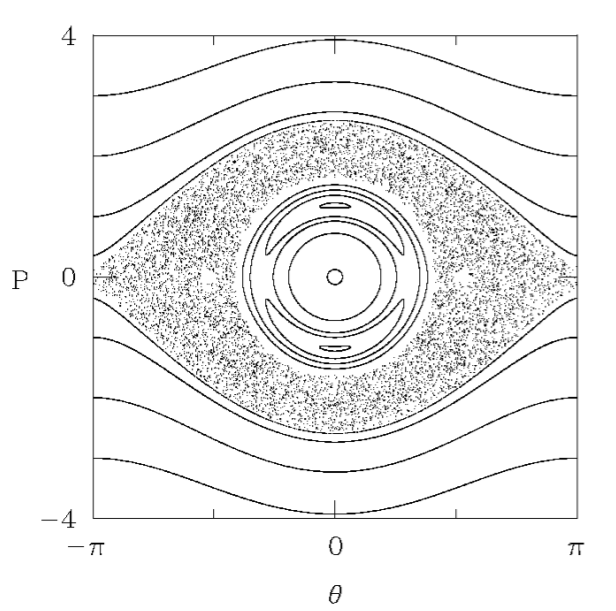
\includegraphics[width=1\linewidth]{./01_1.png}
\end{minipage}
\end{figure}
\end{frame}

\begin{frame}{The role of chaotic resonances in the solar system (2001)}
\begin{figure}[h]
\begin{minipage}[h]{0.7\linewidth}
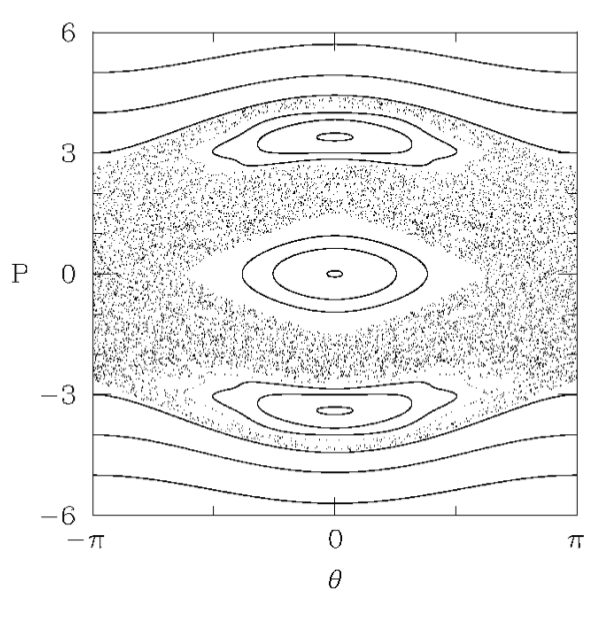
\includegraphics[width=1\linewidth]{./01_2.png}
\end{minipage}
\end{figure}
\end{frame}


\begin{frame}{Chaos in the Solar System (2001)}
        \textbf{Авторы}: Myron Lecar, Fred A Franklin, Matthew J Holman, Norman W Murray.

        \textbf{Кратко}: Физические основы хаоса в солнечной системе -- наложение орбитальных резонансов. Как ярчайший пример -- главный пояс астероидов. Там наложение резонансов даёт известные Люки Кирквуда. Также есть доказательства существования очень узких щелей во внешнем поясе. Пояс Койпера и короткопериодичные кометы. Во внутренней солнечной системе Меркурий из-за наложения нескольких резонансов на временах порядка $10^{12}$ лет может иметь замкнутую орбиту с Венерой (либо упадет на Солнце). Во внешней солнечной системе трехтельный резонанс тоже источник хаоса, но на значительно более долгих временах.

\end{frame}

\begin{frame}{Chaos in the Solar System (2001)}
        Основные выводы:
        \begin{itemize}
                \item Солнечная система нестабильна.
                \item Главной задачей стояло найти накладывающиеся резонансы, порождающие хаос и предсказать время выброса как функцию времени Ляпунова. 
                \item Сеть Арнольда не годится для объяснения хаоса в солнечной системе, интересна как математическая теория. Вековые колебания больших полуосей не могут вызрать нестабильность в таком виде.
                \item Предлагают разделять "сильный" и "слабый" хаос.
        \end{itemize}
        Много красивых картинок
\end{frame}


\begin{frame}{Is the outer Solar System chaotic? (2007)}
        \textbf{Автор}: Wayne B. Hayes

        \textbf{Кратко}: Текущих наблюдений не хватает для ответа на этот вопрос. Показано, что, учитывая ошибки наблюдений, существует протяженная шкала времен Ляпунова для тел внешней солнечной системы от 5 Млет до бесконечности, и время Ляпунова для этого региона не может быть уточнено используя наблюдения, имеющиеся сегодня.
\end{frame}


\begin{frame}{Is the outer Solar System chaotic? (2007)}
        \begin{itemize}
                \item Моделирование по 8 телам (Плутона там нет)
                \item Внутренние планеты преобразованы в точку в барицентре
                \item Сетка на $10^{11}$a элементов, времена интегрирования около 1Глет.
                \item Только Ньютоновская динамика!
                \item Массы объектов константны
                \item Интегратор Cowell-Steormer (14-й порядок)
        \end{itemize}
\end{frame}

\begin{frame}{Is the outer Solar System chaotic? (2007)}
        Начальные условия: JPL's DE405 эфемериды (на тот момент самые авторитетные).
\begin{figure}[h]
\begin{minipage}[h]{0.8\linewidth}
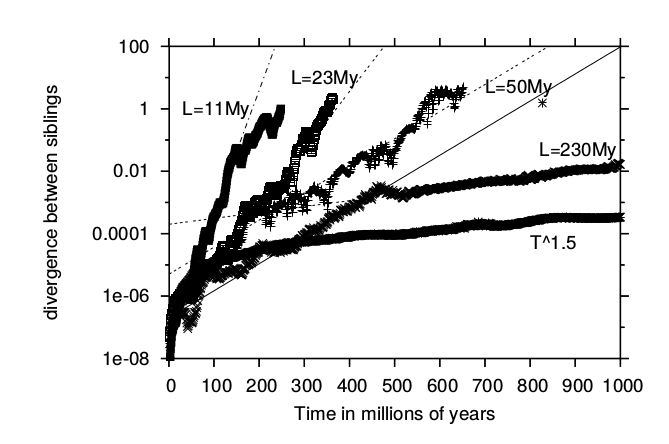
\includegraphics[width=1\linewidth]{./07_1.png}
\end{minipage}
\end{figure}
\end{frame}

\begin{frame}{Theory of Secular Chaos and Mercury's Orbit (2010)}
        \textbf{Авторы}: Yoram Lithwick, Yanqin Wu.

        \textbf{Кратко}: Изучали хаотическую эволюцию орбит, фокусируясь на вековых взаимодействиях как наиболее доминирующих на больших шкалах времени. Наложение вековых резонансов приводит к хаосу в планетных системах. Объяснение этого с помощью "map of the mean momenta". Применили этот новый инструмент к Меркурию. Существование Меркурия стоит на пороге хаоса.

\end{frame}

\begin{frame}{Theory of Secular Chaos and Mercury's Orbit (2010)}
        \begin{itemize}
                \item Получены наглядные изображения проявлений хаоса на карте средних моментов
                \item Хаос движения Меркурия разложен на компоненты
                \item Меркурий почти на пороге хаотического движения. Достаточно изменения (уменьшения) наклонения или эксцентриситета одной из планет (Венеры или Юпитера) на $20 - 25$\%, чтобы Меркурий покинул нас через примерно 100 Млет.
        \end{itemize}
\end{frame}

\begin{frame}{Theory of Secular Chaos and Mercury's Orbit (2010)}
\begin{figure}[h]
\begin{minipage}[h]{0.65\linewidth}
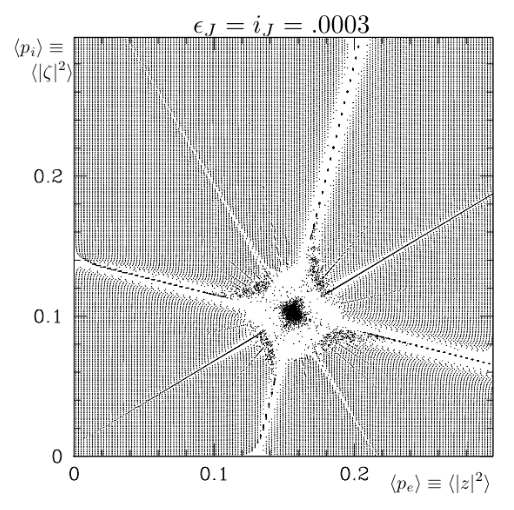
\includegraphics[width=1\linewidth]{./10_1.png}
\end{minipage}
\end{figure}
\end{frame}

\begin{frame}{Theory of Secular Chaos and Mercury's Orbit (2010)}
\begin{figure}[h]
\begin{minipage}[h]{0.65\linewidth}
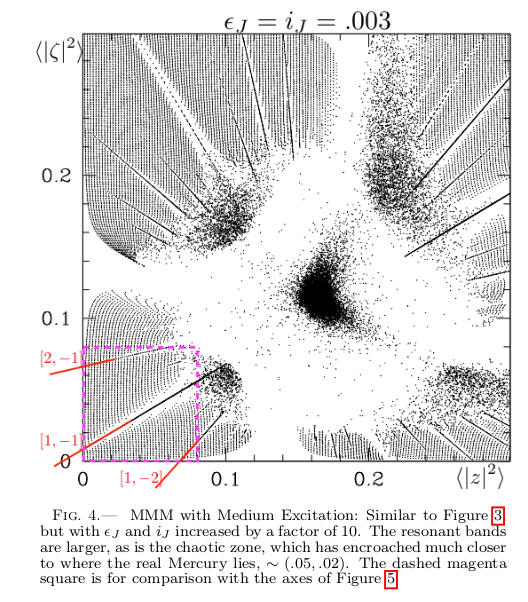
\includegraphics[width=1\linewidth]{./10_2.png}
\end{minipage}
\end{figure}
\end{frame}


\begin{frame}{Theory of Secular Chaos and Mercury's Orbit (2010)}
\begin{figure}[h]
\begin{minipage}[h]{0.65\linewidth}
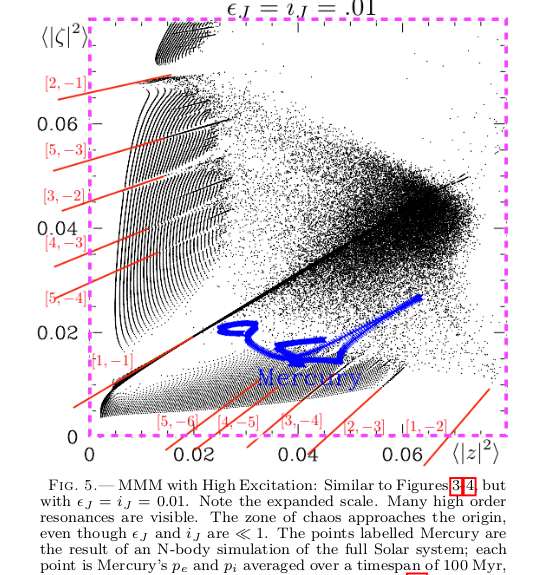
\includegraphics[width=1\linewidth]{./10_3.png}
\end{minipage}
\end{figure}
\end{frame}


\begin{frame}{Theory of Secular Chaos and Mercury's Orbit (2010)}
\begin{figure}[h]
\begin{minipage}[h]{0.65\linewidth}
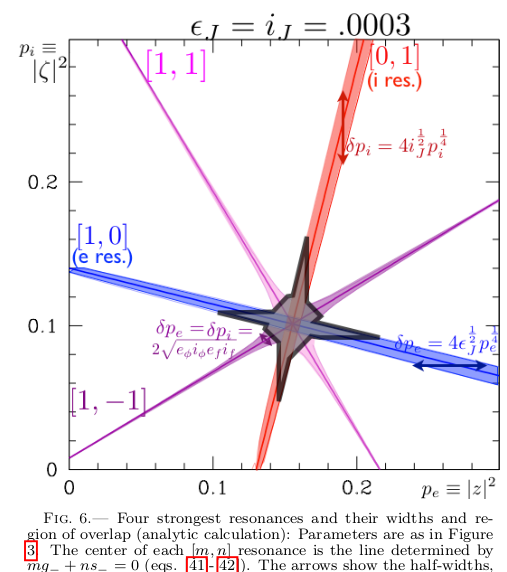
\includegraphics[width=1\linewidth]{./10_4.png}
\end{minipage}
\end{figure}
\end{frame}

\begin{frame}{Theory of Secular Chaos and Mercury's Orbit (2010)}
\begin{figure}[h]
\begin{minipage}[h]{0.65\linewidth}
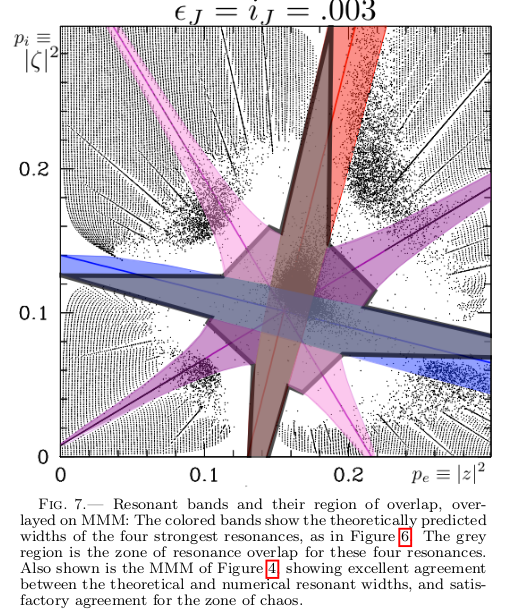
\includegraphics[width=1\linewidth]{./10_5.png}
\end{minipage}
\end{figure}
\end{frame}

\begin{frame}{Theory of Secular Chaos and Mercury's Orbit (2010)}
\begin{figure}[h]
\begin{minipage}[h]{0.65\linewidth}
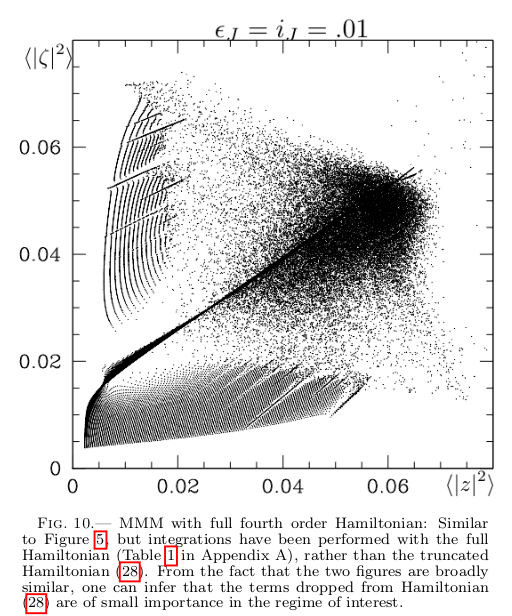
\includegraphics[width=1\linewidth]{./10_6.png}
\end{minipage}
\end{figure}
\end{frame}

\begin{frame}{Secular chaos and its application to Mercury etc (2013)}
        \textbf{Авторы}: Yoram Lithwick, Yanqin Wu.

        \textbf{Кратко}: Существует опасность потерять Меркурий через несколько миллиардов лет. Вековой хаос движет эволюцией солнечной системы сегодня, и помог её создать в прошлом. Мы показали, что внесолнечные планетные системы также формируются по воздействием векового хаоса. Также здесь разъясняем физику векового хаоса и применяем эту теорию к Меркурию и горячим юпитерам.
\end{frame}

\begin{frame}{Secular chaos and its application to Mercury etc (2013)}
\begin{figure}[h]
\begin{minipage}[h]{0.8\linewidth}
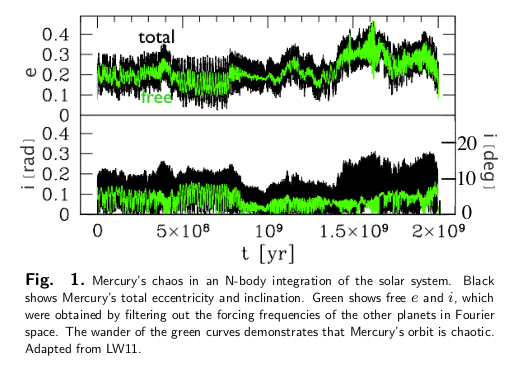
\includegraphics[width=1\linewidth]{./13_1.png}
\end{minipage}
\end{figure}
\end{frame}

\begin{frame}{Secular chaos and its application to Mercury etc (2013)}
\begin{figure}[h]
\begin{minipage}[h]{0.7\linewidth}
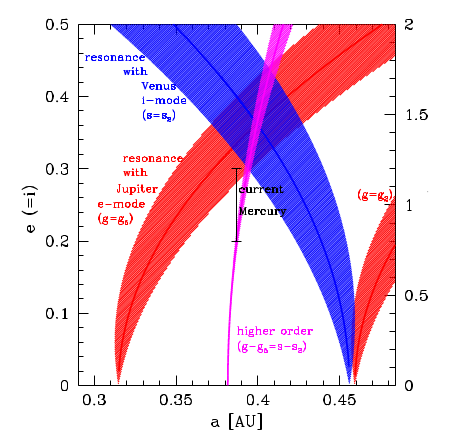
\includegraphics[width=1\linewidth]{./13_2.png}
\end{minipage}
\end{figure}
\end{frame}


\begin{frame}{Chaos in some young asteroid families (2016)}
        \textbf{Авторы}: Rosaev A., Plavalova E.

        \textbf{Кратко}: Исследовались очень молодые астероиды (моложе чем 1Мгод). Показали, что хаос, порожденный резонансами, играет очень важную роль в динамике очень молодых семейств астероидов. Рассмотрены: семейство Datura (резонанс 9:16 с Марсом), Hobson (вековые резонансы), и Kap'bos (причина хаотической динамикии осталась неизвестной). Также показано, что большие астероиды (Церера, Веста) могут сильно влиять на область хаотического движения.  

\end{frame}



\begin{frame}{Chaos in some young asteroid families (2016)}
        Chaos in \textbf{Datura} family:
\begin{figure}[h]
\begin{minipage}[h]{0.75\linewidth}
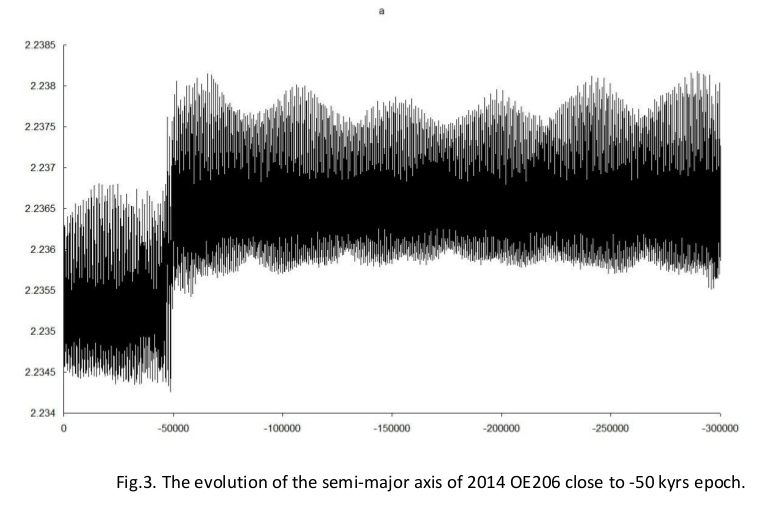
\includegraphics[width=1\linewidth]{./16_1.png}
\end{minipage}
\end{figure}
\end{frame}

\begin{frame}{Chaos in some young asteroid families (2016)}
        Chaos in \textbf{Hobson} family:
\begin{figure}[h]
\begin{minipage}[h]{0.9\linewidth}
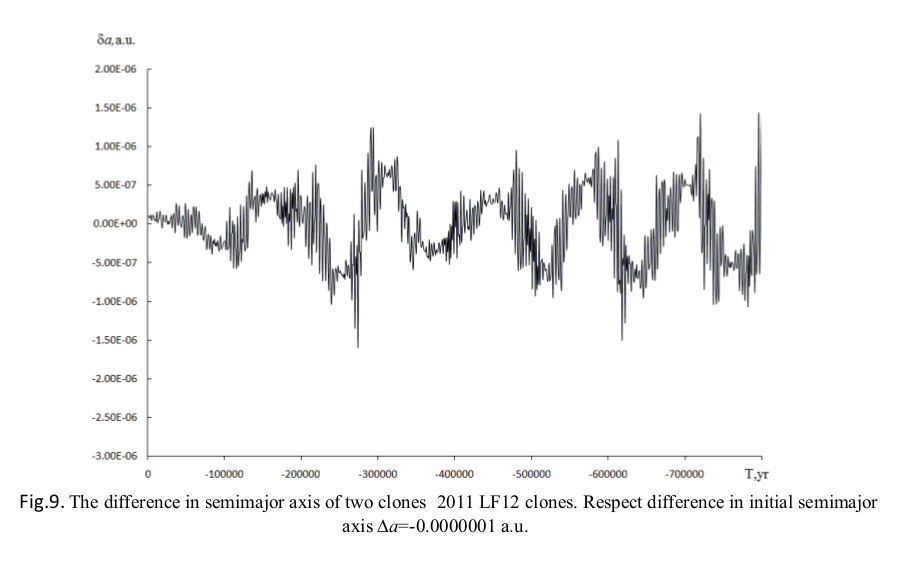
\includegraphics[width=1\linewidth]{./16_2.png}
\end{minipage}
\end{figure}
\end{frame}

\begin{frame}{Chaos in some young asteroid families (2016)}
        Chaos in \textbf{Kap'bos} family:
\begin{figure}[h]
\begin{minipage}[h]{0.8\linewidth}
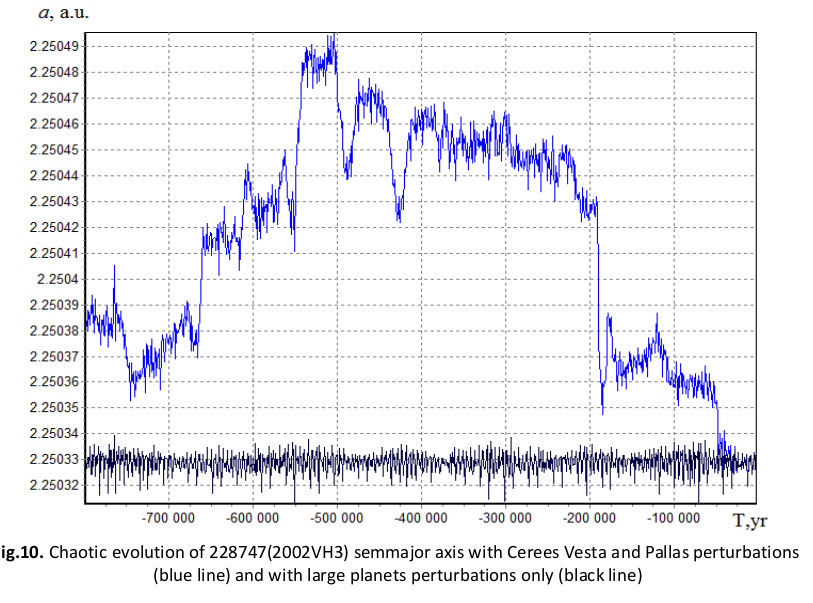
\includegraphics[width=1\linewidth]{./16_3.png}
\end{minipage}
\end{figure}
\end{frame}

\begin{frame}{Chaos in some young asteroid families (2016)}
        Chaos in \textbf{Kap'bos} family:
\begin{figure}[h]
\begin{minipage}[h]{0.8\linewidth}
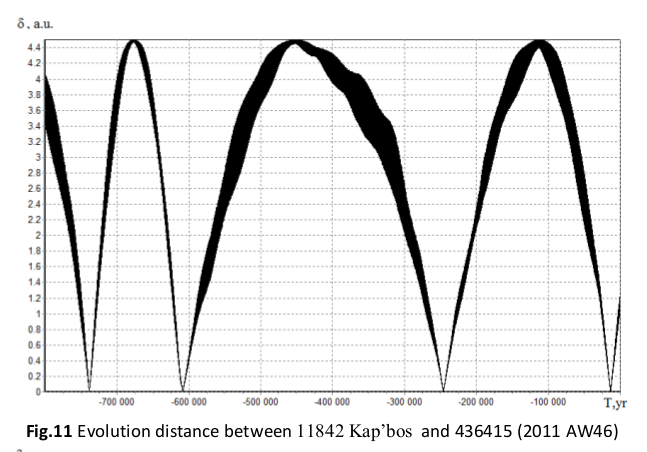
\includegraphics[width=1\linewidth]{./16_4.png}
\end{minipage}
\end{figure}
\end{frame}

\begin{frame}{Chaos in some young asteroid families (2016)}
        Chaos in \textbf{Kap'bos} family:
\begin{figure}[h]
\begin{minipage}[h]{0.8\linewidth}
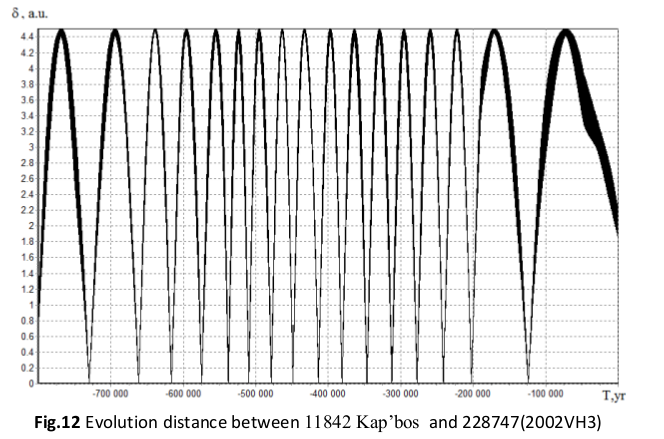
\includegraphics[width=1\linewidth]{./16_5.png}
\end{minipage}
\end{figure}
\end{frame}

\begin{frame}{Chaos in some young asteroid families (2016)}
        Chaos in \textbf{Kap'bos} family:
\begin{figure}[h]
\begin{minipage}[h]{0.8\linewidth}
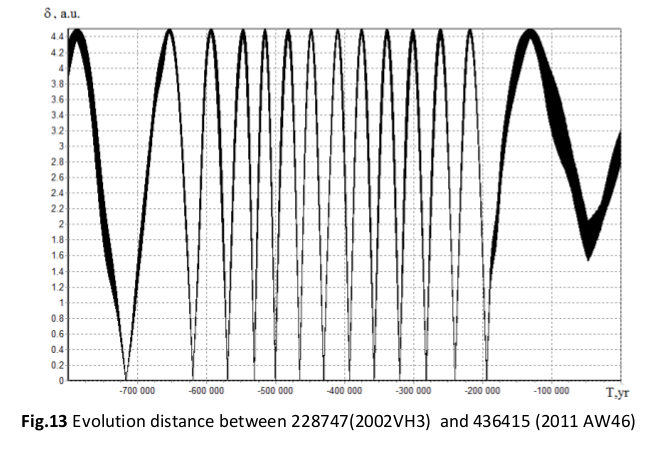
\includegraphics[width=1\linewidth]{./16_6.png}
\end{minipage}
\end{figure}
\end{frame}






\begin{frame}{Ссылки}
        Помимо вышеупомянутыx работ для подготовки использовалась статья А.Ю.Лоскутова "Очарование хаоса" (Dec. 2010, УФН)
\end{frame}


\end{document}

